\section{1042 --- Flower Planting With No Adjacent (LeetCode)}

\subsection*{Código}
\lstinputlisting{1042_FlowerPlanting.java}

\subsection*{Comprovante de aceite}
\begin{center}
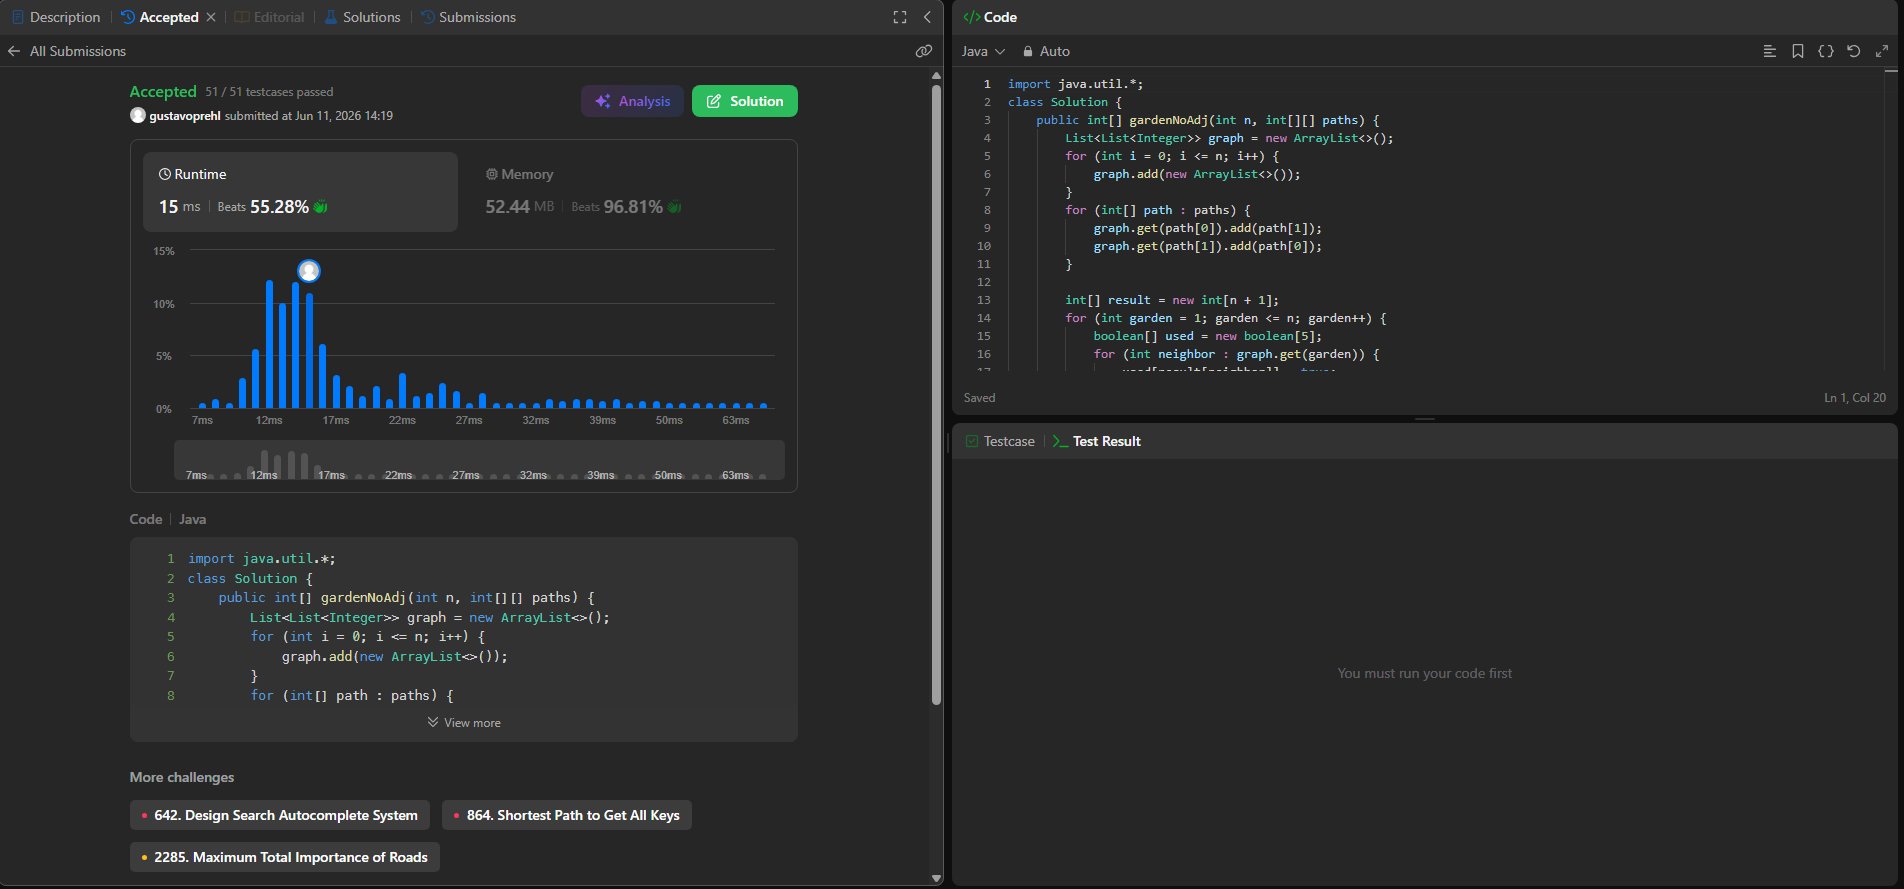
\includegraphics[width=0.85\textwidth]{Accepts/1042_FlowerPlanting_Submit.png}\\
\end{center}

\subsection*{Justificativa}

\textbf{Estratégia:} coloração gulosa de grafos.

O problema é equivalente a colorir os vértices de um grafo (jardins =
vértices, caminhos = arestas) de forma que vértices adjacentes recebam cores
diferentes, usando até 4 cores (tipos de flores).

\textbf{Por que 4 cores sempre bastam (correção):} a restrição garante que
cada vértice tem grau no máximo 3 (no máximo 3 caminhos incidentes). Pelo
teorema da coloração gulosa, qualquer grafo pode ser colorido com no máximo
$\Delta + 1$ cores, onde $\Delta$ é o grau máximo --- basta processar os
vértices em qualquer ordem e, para cada um, atribuir a menor cor que ainda
não foi usada por nenhum de seus vizinhos já coloridos. Como
$\Delta \leq 3$, sempre haverá pelo menos uma cor livre entre as 4
disponíveis, mesmo que todos os vizinhos já coloridos usem cores distintas
entre si.

\textbf{Implementação:} constrói-se a lista de adjacência a partir de
\texttt{paths} e, para cada jardim de 1 a $n$, marca-se em um vetor booleano
\texttt{used[1..4]} quais cores já foram usadas pelos vizinhos processados
anteriormente; a primeira cor livre é atribuída ao jardim atual.

\textbf{Complexidade:}
\begin{itemize}
    \item Tempo: $O(n + |paths|)$ --- a construção do grafo é $O(|paths|)$ e
    a coloração visita cada vértice e cada aresta um número constante de
    vezes (grau $\leq 3$).
    \item Espaço: $O(n + |paths|)$ para a lista de adjacência e o vetor de
    resultado.
\end{itemize}

\textbf{Tópico do curso:} coloração gulosa baseada no teorema $\Delta + 1$
--- \emph{Estratégia Gulosa e Divisão e Conquista} [CLRS09, caps. 4 e 16].
Como o algoritmo resolve o problema em tempo polinomial $O(n + |paths|)$, ele
também ilustra a \emph{Classe P} [CLRS09, cap. 34.1].
